\chapter{Trajectory Determination Techniques}
\label{ch:trajectory}
As discussed in the previous chapter, after a full sequence of image processing, the system obtains the location of the centroid of the target. As determination of distance is unfeasible, this location is given in terms of exclusively angular measurements. Therefore, to determine the trajectory, the problem reduces to determining the trajectory of the target through purely angular measurements. The reader is encouraged to ponder over this statement for a moment, as its inherent challenges form the basis of this chapter.\\

Trajectory determination is a wide and often studied field, with applications in for example sports (\cite{trajtwo}), industry (\cite{anntrajectoryone}, \cite{trajone}, \cite{trajthree}), defense (\cite{anntrajectoryone}) and more close to the area of research: in meteor trajectories in Earth's atmosphere (e.g. \cite{trajfour}, \cite{trajfive}, \cite{trajsix}) and orbits of satellites (\cite{phddissertation}). The promising methods have been compiled into this section as a suggestion on the future research methods. Firstly, some methods specific to orbits are discussed, such as Gauss' method. Then, more general techniques which can be applied to this problem are explained. The actual implementation of them, however, is beyond the scope of this report.

\section{Gauss' Method}
\label{sec:gaussmethod}
The first to attempt a solution to this problem was \cite{gaussceres}. Gauss applied his method to solve for the orbit of the dwarf planet Ceres, discovered a few years prior. Its position was known only at each instant $n$ only in terms of right ascension $\alpha_n$ and declination $\delta_n$, and thus also the unit vector $\hat{\rho}_n$ from the observation point to the orbiting body could be defined. Gauss' method has been replaced by more accurate methods, but the ideas in it are fundamental enough to warrant inclusion in this report. \\

Taking three observations, Gauss' method is performed as follows (\cite{curtis}). Firstly, define timesteps:
\begin{align}
    \tau_1 &= t_1 - t_2 \\
    \tau_3 &= t_3 - t_2 \\
    \tau &= t_3 - t_1
\end{align}
Then, take the vector products of the unit vectors:
\begin{align}
    \vec{P_1} &= \hat{\rho}_2 x \hat{\rho}_3 \\
    \vec{P_2} &= \hat{\rho}_1 x \hat{\rho}_3 \\
    \vec{P_3} &= \hat{\rho}_1 x \hat{\rho}_2
\end{align}
Calculate ten scalar quantities. $D_0$ the triple product of the unit vectors, and $D_{11}$ through $D_{33}$ following from the product of the $\vec{P}_n$ with the observers position vector at time of observation $\vec{R}_n$
\begin{equation}
    D_{mn} = \vec{R}_m \cdot \vec{p}_n
\end{equation}
From this, calculate the following polynomial coefficients:
\begin{align}
    a &= -\left(A^2 + 2AE + R_2^2\right) \\
    b &= -2\mu B\left(A + E\right) \\
    c &= \mu^2 B^2
\end{align}
with:
\begin{align}
    A &= \frac{1}{D_0}\left(-D_{12}\frac{\tau_3}{\tau} + D_{22} + D_{32}\frac{\tau_1}{\tau}\right) \\
    B &= \frac{1}{6D_0}\left( D_{12} \left(\tau_3^2 - \tau^2\right)\frac{\tau_3}{\tau} + D_{32}\left( \tau^2 - \tau_1^2\right)\frac{\tau_1}{\tau}\right) \\
    E &= \vec{R}_2 \cdot \hat{\rho}_2 \\
    R_2^2 &= \vec{R}_2 \cdot \vec{R}_2
\end{align}
Then, the polynomial
\begin{equation}
    r_2^8 + a_2^6 + b_2^3 + c = 0
    \label{eq:gausspolynomial}
\end{equation}
Can be solved for the scalar distance to the target at time 2. From here, the slant range and slant position vector can be calculated easily through vector operations. This yields the position vectors $\vec{r}_n$ of the target at the times of observation. From this, the first two terms of the Lagrange series can be determined:
\begin{align}
    f_1 &\approx 1- \frac{1}{2}\frac{\mu}{r_2^3}\tau_1^2 \\
    f_3 &\approx 1-\frac{1}{2}\frac{\mu}{r_2^3}\tau_3^2 \\
    g_1 &\approx \tau_1 - \frac{1}{6}\frac{\mu}{r_2^3}\tau_1^3 \\
    g_3 &\approx \tau_3 - \frac{1}{6} \frac{\mu}{r_2^3}\tau_3^3
\end{align}
And the velocity of the target follows from:
\begin{equation}
    \vec{v}_2 = \frac{1}{f_1g_3 - f_3g_1}\left(-f_3\vec{r}_1 + f_1 \vec{r}_3\right)
\end{equation}
The position and velocity vector of the target have been found, and therefore the orbit has been determined. From here, methods exist to improve the accuracy through small corrections. Although this process in itself is not very interesting for the research, it is important to discuss its assumptions and how these make it infeasible. In particular: the estimation of the Lagrange coefficients is not very accurate, the solution assumed a two-body motion and the solution is very sensitive to errors in the initial measurements in the case of a very short arc, as shown by \cite{classicmodernorbits} in \autoref{fig:gaussshortarc}: the initial error in measurement causes a completely erroneous estimate.

\begin{figure}[htbp]
    \centering
    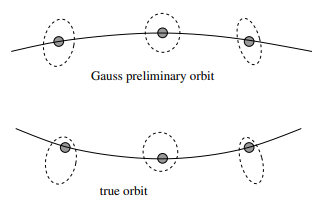
\includegraphics[width=0.5\textwidth]{images/gausstruearc.png}
    \caption{Actual orbit and orbit as determined by Gauss' method for a short arc}
    \label{fig:gaussshortarc}
\end{figure}

Several of the estimation problems can be resolved, e.g. through the methods proposed by \cite{anglesonly}. Der postulates that the efficacy of initial orbit determination might be improved through elimination of numerically sensitive methods such as numerical integration of higher order partial derivatives, inversions of matrices or certain iterative methods. Firstly, the roots of \autoref{eq:gausspolynomial} might be determined rather than guessed through application of logic (e.g. on what side of the Sun is the orbit going to be). Secondly, instead of determining or guessing a single range vector, $\vec{r}_2$, it is possible to instead solve for $\vec{r}_1$ and $\vec{r}_3$. This reduces the problem to Lambert's problem: determine the orbit from two range vectors and time of flight, for which a solution exists (for more information, refer to \cite{curtis}). Lastly, it is possible to solve the Lambert problem for perturbed orbits (e.g. \cite{superlambert} and \cite{superlamberttwo}) using modern numerical algorithms. The accuracy of the resulting calculation is dependent on the measurements, as discussed earlier. For a good set of measurements, Der recommends spacing the measurements by several days to months, but within a single orbit. In addition, the accuracy of the measurement should be in the order of 5 significant digits or better. three to four significant digits might yield "acceptable" results, anything less will result in unusable results. For the intended research, the angular resolution is not an inherent problem, although the observation window might be. Therefore, methods applicable to shorter arcs should also be considered.

\section{The Method of Very Short Arcs}
The theory on trajectory determination for very short arcs was first introduced by \cite{veryshortarcs}, who worked out the solutions in more detail in subsequent papers (e.g. \cite{veryshortarcstwo}). Starting from fundamentals, define a \textit{sequence of observations} as a set of observations belonging to the same object:
\begin{equation}
    t_i,~\alpha_i,~\delta_i,~h_1;~i = 1, 2, ..., m;~m \geq 2
\end{equation}
With:
\begin{itemize}
    \item $t_i$: time of the observation.
    \item $\alpha_i, \delta_i$: right ascension and declination at time $t_i$.
    \item $h_i$: apparent visual magnitude (optional)
\end{itemize}
These observations can be said to belong to the same object if they allow construction of a \textit{very short arc}: the observations are close enough together that they can be fit to some smooth curve (\cite{classicmodernorbits}). From here, a vector shall be defined as \textit{attributable} if:
\begin{equation}
    \xi = (\alpha, \delta, \dot{\alpha}, \dot{\delta})~\in~[-\pi, \pi)~\times~(-\pi/2, \pi/2)~\times~\mathbb{R}^2
\end{equation}
If the apparent magnitude is available, it is also included in the attributable. If the arc described by the observations does not allow for a convergent estimation of the orbit using a classical method as described in \autoref{sec:gaussmethod}, the arc is termed a \textit{too short arc}. In this case, it is important to note that the quantities of interest, namely the position and velocity $r$ and $\dot{r}$ are completely undetermined. In this case, an attributable can still be used to perform several operations:
\begin{itemize}
    \item The attributable can be \textit{attributed} to a known object with a known orbit using a least-squares estimation. This essentially identifies the attributable as belonging to that object.
    \item The attributable can be \textit{linked} to another attributable of (possibly) the same object. This lengthens the arc and might allow orbit computation
    \item The attributable can be linked to a new attributable from an object in the sky (\text{recovery}) or the archives (\textit{precovery}), by the same logic as the previous point.
\end{itemize}
It might seem like the possibilities end here. However, it is possible to couple the information from the attributable to information on the population of the objects of interest. \cite{veryshortarcs} describe this process for observations of targets in heliocentric orbits from Earth, but the process is easily adapted. Milani et al. define the \textit{admissible region} as the subset of $(r, \dot{R})~\in~\mathbb{R}^2$ for which the following holds:
\begin{enumerate}
    \item The target is not in an orbit around Earth, i.e. $\mathcal{E}_\oplus (r, \dot{r}) \geq 0$. This is only useful if:
    \item The object is inside the sphere of influence of Earth: $r \leq 0.01044 AU$.
    \item The object is not interstellar: $\mathcal{E}_\odot (r, \dot{r}) \leq 0$.
    \item The object is not very small (and thus very close): $H \leq H_{max}$ for some reasonable value of $H_{max}$.
\end{enumerate}
Logically, it follows that the admissible region is thus defined as $\left[ (\mathbf{1}) \cup (\mathbf{2})^c\right] \cap (\mathbf{3}) \cap \mathbf{4}$, which is shown qualitatively in \autoref{fig:admissibleregion}.
\begin{figure}[htbp]
    \centering
    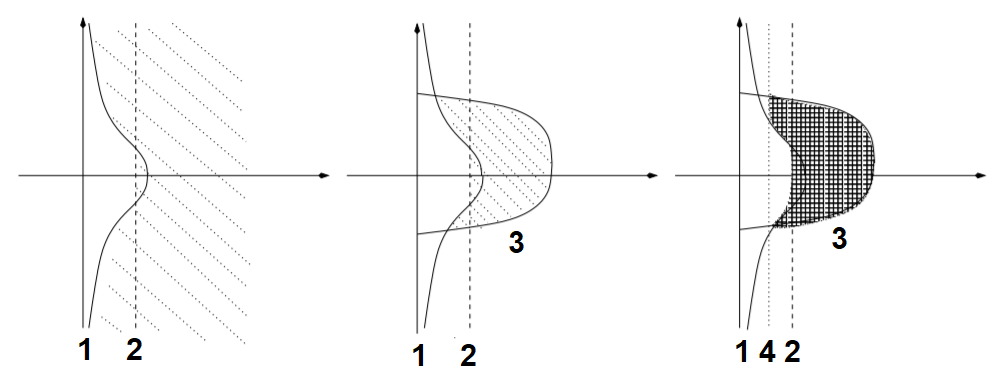
\includegraphics[width=0.7\textwidth]{images/admissibleregoin.png}
    \caption{Sketch of the construction of the admissible region (\cite{classicmodernorbits}).}
    \label{fig:admissibleregion}
\end{figure}
Importantly, the concept of \textit{admissible region} can be adapted to the purpose of potentially hazardous near-Earth asteroids quite easily. Most obviously, using \autoref{eq:sizealbedo}, a reasonable value of $H_{max}$ can be determined. The computation of absolute from apparent magnitude follows readily from the average apparent magnitude $h^{*}$, allowing a constraint on the radius vector:
\begin{equation}
    H = h^* - h \log_{10} r - x(r)
\end{equation}
In addition, condition $\mathbf{1}$ can be adjusted to fit objects with a certain range of semi-major axes:
\begin{equation}
    -\frac{\mu_\odot}{2a_{min}} \leq \mathcal{E}_\odot \leq -\frac{\mu_\odot}{2a_{max}}
\end{equation}
From here, it becomes possible to simulate the entire subspace of \textit{virtual asteroids}. \autoref{fig:admissibleexample} shows this region, with a selection of virtual asteroids triangulated on it. Each of these asteroids has a fully determined set of orbital elements, which can be propagated into the past and future for operations such as linkage, or to determine the possibility of the asteroid being on an impact trajectory with Earth. This can be done with e.g. an analogue to the method suggested by \cite{trajsix} or with a least-squares based approach such as suggested by \cite{phddissertation}.

\begin{figure}[htbp]
    \centering
    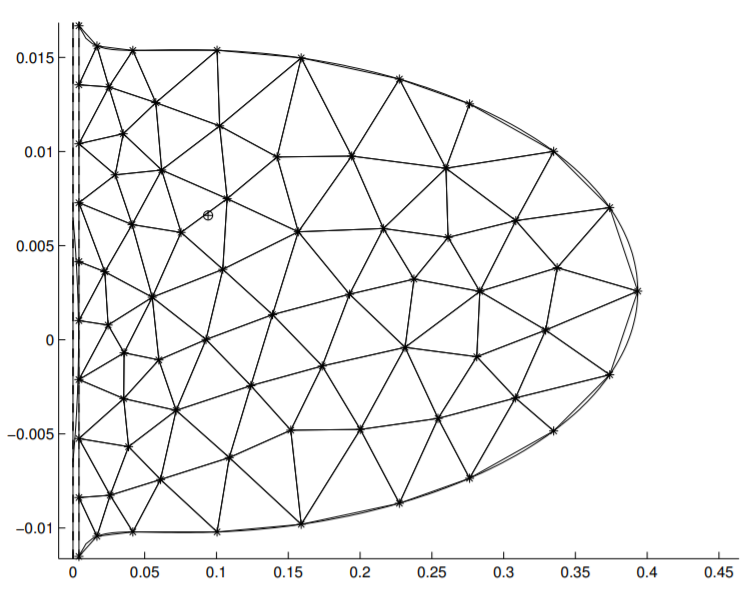
\includegraphics[width=0.5\textwidth]{images/admissibleexample.png}
    \caption{An example of an admissible region, for asteroid $2003 BH_{84}$ using exclusively data from the day of first observation. The vertical axis is $\dot{r}$[AU/day], the horizontal axis is $f(r) = 1-e^{-r^2/(2s^2)}$ where $s$ is a normalization term. The real position of the asteroid is marked near the top left with a $\oplus$. (\cite{classicmodernorbits})}
    \label{fig:admissibleexample}
\end{figure}

\section{Kalman Filters}
Kalman filters (KF) are an essential component of modern control theory and nonlinear state estimation (\cite{kalmangood}). The idea of a Kalman filter was first described by \cite{kalman}. The Kalman filter or linear quadratic estimator (LQE) provides the optimal linear estimation for linear systems with gaussian (white) noise. The KF algorithm is a recursive estimator based around two alternating steps: predict and update.\\

Firstly, in the predict step, the filter produces an a priori estimate of the evolution of the state based on the current state and any inputs. In addition, the covariance of the state is estimated. Then, in the update step, the predicted state is compared with a measurement. This is known as the innovation residual. Using this innovation residual, a gain is calculated for the correction of the state estimate and covariance. Then, the state is updated and the filter goes back to the predict step.\\

Firstly, the following are defined:
\begin{itemize}
    \item $\vec{x}_k$: the state vector of the system.
    \item $\vec{u}_k$: the control-input vector (most likely $\vec{0}$ for the proposed application)
    \item $\vec{w}_k$: the process noise, which is assumes to follow a normal distribution with covariance $\mathbf{Q}_k$: $\vec{w}_k\sim\mathcal{N}(0, \mathbf{Q}_k$. This represents any perturbation in the trajectory not accounted for in the state-transition.
    \item $\mathbf{F}_k$: the state-transition matrix.
    \item $\mathbf{B}_k$: the control-input model.
\end{itemize}
Such that the state at time $k$ is determined from the state at time $k-1$:
\begin{equation}
    \vec{x}_k = \mathbf{F}_k \vec{x}_{k-1} + \mathbf{B}_k \vec{u}_k + \vec{w}_k
\end{equation}
Then, the system will make an observation at time $k$ with the following:
\begin{itemize}
    \item $\vec{z}_k$: the observation vector.
    \item $\vec{v}_k$: the observation noise, assumed to be $\vec{v}_k\sim\mathcal{N}(0, \mathbf{R}_k)$ with covariance $\mathbf{R}_k$.
    \item $\mathbf{H}_k$: the observation model, responsibly for mapping the state space onto the observation space.
\end{itemize}
Lastly, there are two important state variables for the filter:
\begin{itemize}
    \item $\hat{x}_{k|k}$: the a posteriori state estimate at time $k$ from the observation at time $k$ and all preceding observations.
    \item $\mathbf{P}_{k|k}$: the a posteriori coviarance matrix estimate, which is importantly a measure of the accuracy of the prediction.
\end{itemize}
Using the notation $\hat{x}_{n|m}$ being the estimate of $\vec{x}$ at time $n$ by all observations preceding and including the observation at time $m$, the full filter can be expressed as:\\

\begin{centering}
Prediction step:
\begin{align}
    \hat{x}_{k|k-1} &= \mathbf{F}_k\hat{x}_{k-1|k-1} + \mathbf{B}_k\vec{u}_k\\
    \mathbf{P}_{k|k-1} &= \mathbf{F}_k\mathbf{P}_{k-1|k-1}\mathbf{F}_k^T+\mathbf{Q}_k
\end{align}
Update step:
\begin{align}
    \bar{y}_k &= \vec{z}_k - \mathbf{H}_k\hat{x}_{k|k-1} \\
    \mathbf{S}_k &= \mathbf{H}_k\mathbf{P}_{k|k-1}\mathbf{H}_k^T + \mathbf{R}_k \\
    \mathbf{K}_k &= \mathbf{P}_{k|k-1}\mathbf{H}_k^T\mathbf{S}_k^{-1} \\
    \hat{x}_{k|k} &= \hat{x}_{k|k-1} + \mathbf{K}_k\bar{y}_k \\
    \mathbf{P}_{k|k} &= \left(\mathbf{I} - \mathbf{K}_k\mathbf{H}_k\right)\mathbf{P}_{k|k-1} \\
    \bar{y}_{k|k}&= \vec{z}_k - \mathbf{H}_k\hat{x}_{k|k}
\end{align}
\end{centering}

At this point, it is good to note that the Kalman filter provides to optimal estimation for \textbf{linear} systems with \textbf{zero-mean, independent Gaussian} noise. Of course, in reality these assumptions are not valid, and inaccurate modeling of the system dynamics can lead to disastrous results (\cite{EKF}). Therefore, the Extended Kalman Filter (EKF) might provide a useful solution. In the EKF, the system is linearized about the estimate of the current mean and covariance. It is considered the standard in nonlinear state estimation (\cite{kalmangood}).\\

The EKF is a generalization of the standard Kalman filter by means of linearization of the state and observation models (\cite{extendedkalman}). At the cost of no longer representing the optimal estimator, the EKF allows for the state-transition and observation matrices to instead be differentiable functions $f$ and $h$, such that:
\begin{align}
    \vec{x}_k &= f(\vec{x}_{k-1}, \vec{u}_k) + \vec{w}_k
    \label{eq:extendedstate} \\
    \vec{z}_k &= h(\vec{x}_k) + \vec{v}_k
    \label{eq:extendedobservation}
\end{align}
The functions $f$ and $h$ allow for these transformations to be made. However, they can not be used to recompute the estimate of the covariance. Therefore, the Jacobian of the functions is used instead:
\begin{equation}
    \frac{\partial f}{\partial \vec{x}} = \mathbf{J}_f(\vec{x}) = \begin{bmatrix} \frac{\partial f_1}{\partial x_1} & \cdots & \frac{\partial f_1}{\partial x_n} \\
    \vdots & \ddots & \vdots \\
    \frac{\partial f_m}{\partial x_1} & \cdots & \frac{\partial f_m}{\partial x_n} \end{bmatrix}
    \label{eq:jacobian}
\end{equation}
Thus, after substitution of \autoref{eq:extendedstate} and \autoref{eq:extendedobservation} into the standard Kalman filter, the remaining state and observation matrices can be approximated by the following Jacobians:
\begin{align}
    \mathbf{F}_k &\approx \left \frac{\partial f}{\partial \vec{x}} \right|_{\hat{x}_{k-1|k-1}, \vec{u}_k} \\
    \mathbf{H}_k &\approx \left \frac{\partial h}{\partial \vec{x}} \right|_{\hat{x}_{k|k-1}}
\end{align}

Kalman filters are a promising technique for performing the further research. For example, \cite{trajectorythesis}, shows very good results in approximating trajectories using an Extended Kalman Filter, but does note that the filter has problems when the trajectory deviates too much from the used physics model. Therefore, finding a good linearized representation is essential.

\section{Artificial Neural Networks}
\label{sec:ANN}
\begin{figure}[htbp]
    \centering
    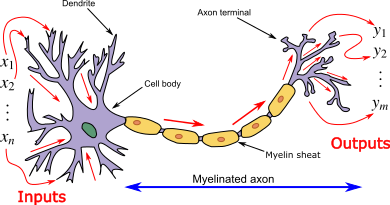
\includegraphics[width=0.6\textwidth]{images/neuron.png}
    \caption{Comparison of a biological neuron with an artificial neuron. The Neuron takes inputs, combines those, and forwards them to produce a set of outputs. Note that this is where the analogy ends: biological neurons behave very differently to ANN's. CC BY-SA 4.0 Prof. Vu-Quoc.}
    \label{fig:bioneuron}
\end{figure}
Artificial neural networks (ANN's) are a class of Machine Learning - or popularly \textit{Artificial Intelligence} - models used to perform complex nonlinear tasks that might be impossible, or at best highly unfeasible, to solve using conventional algorithms. ANN's comprise broad functions which are fit to often very large datasets using \textit{learning} algorithms (\cite{nnbooktwo}\footnote{If the reader is interested in learning more about machine/deep learning, this book is highly recommended}). The initial inspiration for ANN's was to very loosely model the neurons in biological brains (see \autoref{fig:bioneuron}), but it should not be seen as being an even remotely accurate representation of biological neural circuitry ( \cite{nnbookone}). \\

In its simplest form, an ANN consists of interconnected neurons. These neurons produce an \textit{activation} $a$ based on the output of neurons connected to it:
\begin{equation}
    a(\vec{o}) = f \left( \Sigma w_io_i + b\right) 
    \label{eq:neuron}
\end{equation}
Here, $o_i$ and $w_i$ represent the output and weight of input neurons respectively, $b$ is a bias term, and $f()$ is an \textit{activation function}. The purpose of this activation function becomes clear once the structure of an ANN is examined in more detail, such as in \autoref{fig:nnstructure}: The input to the network is passed through one of more \textit{hidden layers}, to finally reach an output layer. As any linear combination of linear functions is in itself a linear function, it becomes clear that it is neccessary to apply a non-linear activation function to every neuron; else, the entire network would "collapse" into a linear function (\cite{nnbooktwo}).\\

\begin{figure}[htbp]
    \centering
    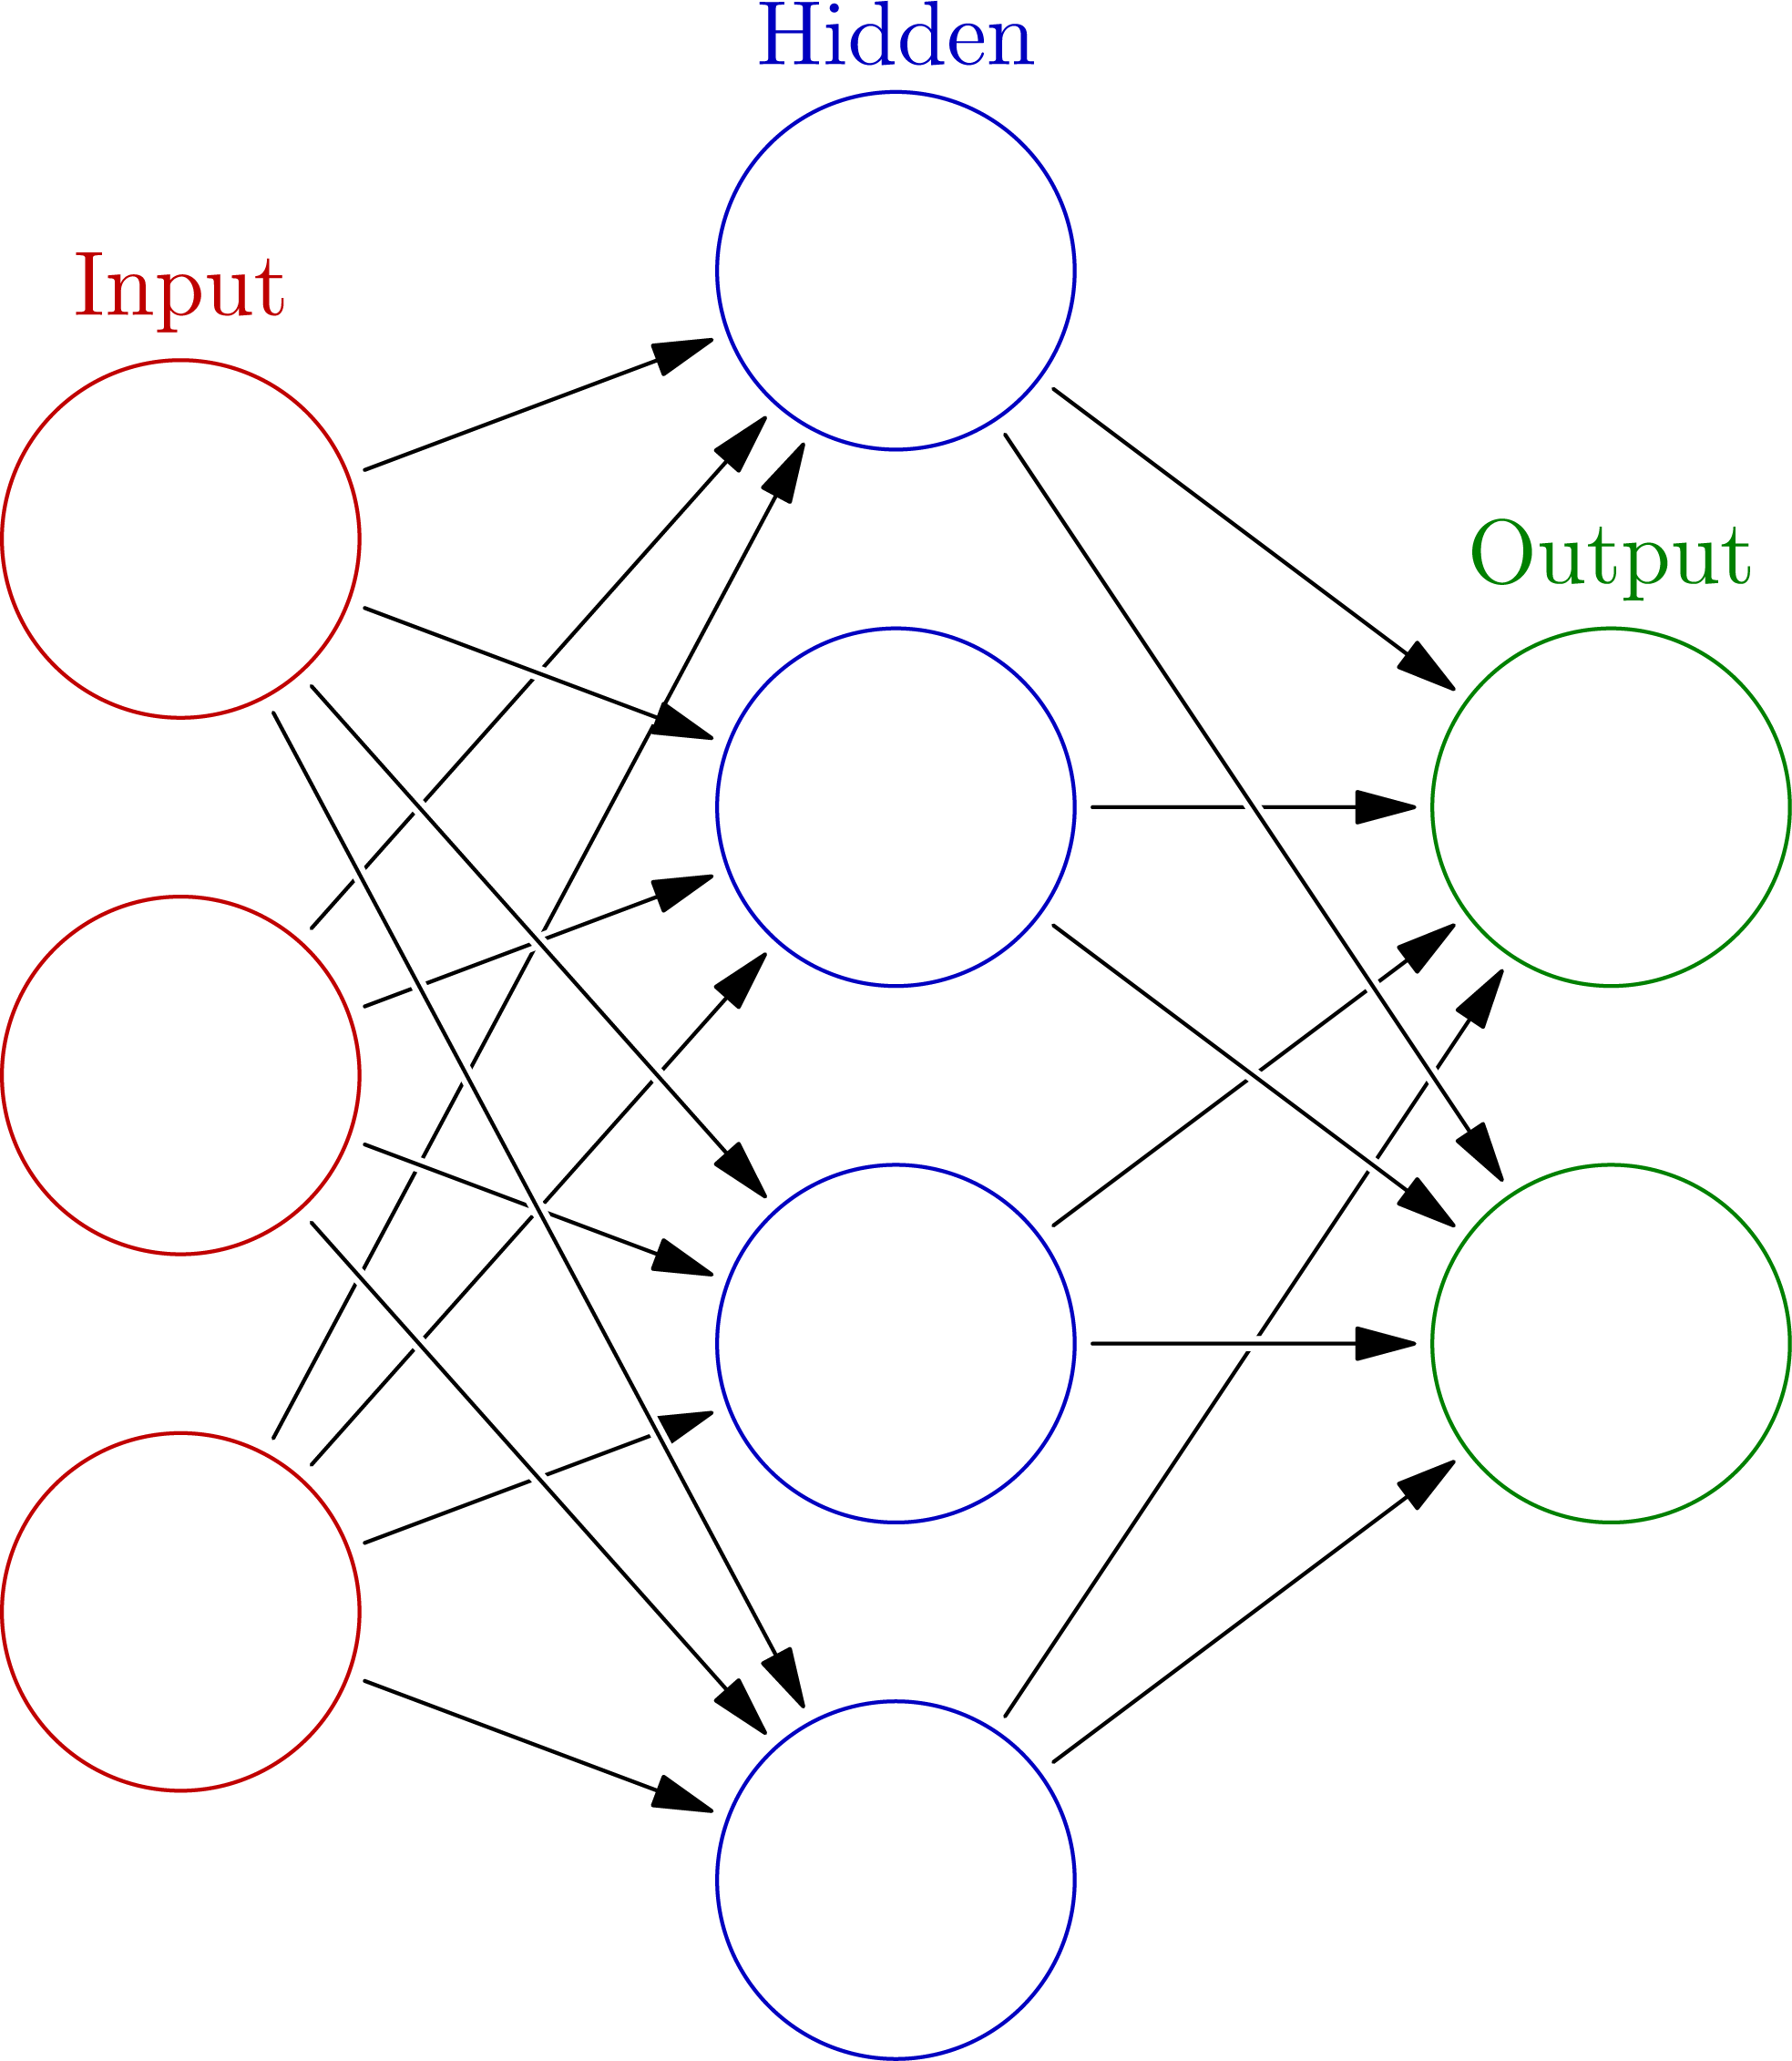
\includegraphics[width=0.4\textwidth]{images/neuralnetwork.png}
    \caption{Structure of a feedforward neural network. CC BY-SA 3.0 Glosser.ca}
    \label{fig:nnstructure}
\end{figure}

In the past, the most commonly used activation function was a sigmoid (an "S"-shape approaching 0 asymptotically as $x \rightarrow -\infty$ and approaching 1 asymptotically as $x \rightarrow \infty$, such as the logistic function (\cite{nnbookfour}):
\begin{equation}
    S(x) = \frac{1}{1+e^{-x}}
\end{equation}
However, as the gradient of the sigmoid function approaches zero for large values of $x$, this presents problems for training. Therefore, a host of different activation functions are used presently. The most commonly used presently are the Rectified Linear Unit (ReLU, \cite{Relu}) and Exponential Linear Unit (ELU, \cite{ELU}):
\begin{align}
    \mathrm{ReLU}(x) &= max(0, x) \\
    \mathrm{ELU}(x) &= max(a(e^x-1), x)
\end{align}
Both of which are extremely simple and fast to compute. The ELU yields slightly better results, but requires finding a good value of $a$. \\

Fitting an ANN to a dataset generally requires two processes: learning, and tuning the hyperparameters. Because of the scope of the research, only supervised learning, where the network is provided with both input and desired output, is described. Learning is carried out by algorithms based on  \textit{backpropagation} (\cite{nnbookthree}) and \textit{gradient descent} (\cite{gradientdescent}). Firstly, the network will process some training data. From the output of the network, the loss function is computed. This are generally well-known metrics such as mean squared error. Then, the backpropagation algorithm iterates backwards through the network, using the chain rule to compute the gradient of the loss function with respect to each network weight. It is important to note that, although not a direct process, the algorithm can compute all gradients in a single pass through the network. Thus, it is computationally very efficient. Then, knowing the gradient, a method like gradient descent can be applied:
\begin{equation}
    \vec{w}_{n+1} = \vec{w}_n - \eta \nabla F(\vec{w_n})
\end{equation}
With \textit{learning rate} $\eta$ (a hyperparameter). Thus, for a small enough learning rate, the solution will converge to a minimum for the loss function. Note that this process does not guarantee reaching the global minimum; it only does this for a convex function, which deep neural networks are generally not. Additionally, learning may become excessively slow on "plateaus" of the loss function. For these reasons, some other optimization algorithms have been designed, most popular among which the Stochastic Gradient Descent (SGD, \cite{sgd}) or the derived ADAM optimizer (\cite{Adam}, \cite{AdamKeras}). \\

Next, the hyperparameters, the properties of the network which can not be learned (e.g. number of layers, number of neurons, learning rate) can be tuned. This is generally an iterative process which involves attempting various combinations using a kind of grid search or random search to determine an optimum (\cite{nnbooktwo}). Great care should be taken to not overfit the data in this process, as will be explained in \autoref{ssec:nnproblems}.

\subsection{Types of Neural Networks to be Used}
Having discussed the base theory, it is good to specifiy which types of ANN's are considered for the research. Because of their properties, and general simplicity, the dense and recurring neural networks have been selected for further investigation. Both of these have already been shown to be usable for trajectory estimation (see e.g. \cite{anntrajectoryone} and \cite{anntrajectorytwo})\\

The dense neural network (DNN) can be seen as the simplest of the ANN's. It consists of one or more layers of densely connected simple neurons as described in the previous sections. This has several advantages: it is simple to set up and computationally lightweight, and training is straightforward (\cite{nnbooktwo}). However, dense neural networks are limited in what they can achieve: they are not translationally invariant (such as convolutional neural networks), nor are they capable of processing sequential information coming in in real time: the size of the input and output must be specified beforehand. \cite{anntrajectoryone} achieves very good results using a DNN.\\

On the contrary, recurring neural networks (RNN's) are capable of holding information that arrives in sequence. They achieve this through feeding the output of a neuron back into itself. Thus, \autoref{eq:neuron} changes to:
\begin{equation}
    a(\vec{o})_t = f(\Sigma w_i o_i + b + a_{t-1})
\end{equation}
Thus, the state of the neuron becomes dependent on the state of the neuron in the previous timestep. This gives the neuron a limited amount of "memory". This is obviously very advantageous for processing sequential data. However, the main drawback becomes apparent when it is considered how RNN's are trained: as the normal backpropagation algorithm does not account for the recursive information flow, it is neccessary to perform a change to the algorithm known as "Backpropagation through time" (\cite{nnbooktwo}). Here, the time-sequence of neurons is "unrolled", and the neurons at different timesteps are treated separately for purposes of calculating the gradient. This leads to the first major problem of RNN's: they are very though to train. A lot of data is needed (thus limiting the size of training steps, as computers have a limited physical memory), and the \textit{vanishing gradients} problem, where the gradients become so small that gradient descent becomes overly slow, becomes a large issue (\cite{nnbookfour}). Interestingly, \cite{trajectorythesis} achieves a very poor performance on a similar problem using RNN's. However, the graphs of the resulting trajectories are extremely erratic, so it is speculated that this is a result of overfitting the training data. Therefore, it is proposed to start with a simple, robust model and work out from there.

\subsection{Common Problems and Pitfalls}
\label{ssec:nnproblems}
As mentioned in the previous section, there are several pitfalls that can be encountered in fitting and training ANN's. The most common problems and some solutions are listed in this section, based on the work of \cite{nnbooktwo}.\\

The first, and most common, problem is overfitting the training data. In this case, the network will "learn" the noise in the dataset, rather than learning the useful patterns embedded therein. Because of the way ANN's are trained, this is an oft-encountered problem. Usually, this problem can be identified by an unreasonably effective result on the training data, alongside a very poor generalization to unseen data. The first solution to this problem is to keep a set of validation data completely separate from the training data, and only using this to validate the training. Care should be taken to not use the validation data for other applications, such as tuning the hyperparameters: in this case, the network will repeatedly "see" the validation data indirectly, possibly leading to it fitting to the unseen data as well. Secondly, a number of regularization methods can be applied. Firstly, L1 or Lasso regression, shrinks very small parameters to zero. This means that a parameter which is inconsequential for the result is no longer included, instead of only being included by a very minor amount - which would lead to an overfit. Conversely, L2 or Ridge regularisation, the large values are penalized. This makes sure no unrealistically high values of coefficients can be present. Lastly, there is the idea of "dropout". Here, in every training step, a few neurons are "dropped out" (i.e. set to 0). This forces the remaining neurons to do the work, thereby making sure that all components of the network contribute to a solution.\\

The second problem is the vanishing or exploding gradients problem. Here, the gradients become excessively small or large during training. Because of how backpropagation works, this is especially an issue for very deep (i.e. many layers) networks. As the gradients become very small or large, training can slow excessively, or the solution can diverge. A part of the solution to this problem is using better activation functions such as ReLU or ELU, as described previously. However, in some cases it might be neccessary to include connections to non-adjacent layers, creating a "shortcut" in the network. \\

Then, there is the problem of \textit{Catastrophic interference}. Here, an ANN spontaneously drops all learned information in favor of new information, essentially overfitting to the last bit of information seen. This manifests as a sudden and dramatic drop in performance during training. This problem is very complex to resolve, and should be accounted for depending on how it manifests. Usually, this is done by placing some restraint on how the model is allowed to be sensitive to new information.\\

Lastly, a remark should be made with regards to the quality of the data: as neural networks are trained exclusively using the data supplied to them, this means their quality is highly dependent on the quality of the data provided. Obviously, providing very bad data will lead to a very badly trained model. However, in generalizing to a solution useful in practice, it is important to also not feed the network unrealistically good data. In this case, the model will seem to perform far better than what can be expected from it in reality. Thus, an assessment of the input data is neccessary to perform a useful evaluation of any ANN-based approach.
